The design of the optical line for the new Laser\_II system of the ATLAS Tile
calorimeter is based on the general scheme implemented for laser calibrations
during LHC RUN I and described in ref.\cite{ref:laser_I}. Laser pulses are used for
simultaneous calibration of the gain of the about 10,000 detector PMTs.
An efficient and stable light distribution system and a very stable and redoundant
system to monitor the light transmitted in different points of the distribution
chain are the main characteristics required for such a calibration system.

Based on the experience with the system used during Run I, some major improvements
were implemented in the new system designed for the LHC run II. They are:
\begin{itemize}
\item a compact design of the optical layout fully included in one single box called
"optics box" in the following (in the Run I system the optical elements were located
into two different boxes optically connected with a liquid fiber, the box with laser
was vertically mounted in the host rack. Now, the new compact box is horizontally
placed);
\item a redundant system for monitoring the light transmitted in different points of
the optical line (ten photodiodes receive light picked-up in three
different points of the optical line, while only 4 diodes were used in the Run I
system to monitor light transmission in two points);
\item a new optical device to mix and to distribute the light to a 400 fiber bundle
serving all the 256 modules of the Tile calorimeter;
\item a new anti-vibration suspension system to hold the optics box in a rack of the
service room in the ATLAS cavern.   
\end{itemize}
% 
\begin{figure}[htb]
\begin{center} 
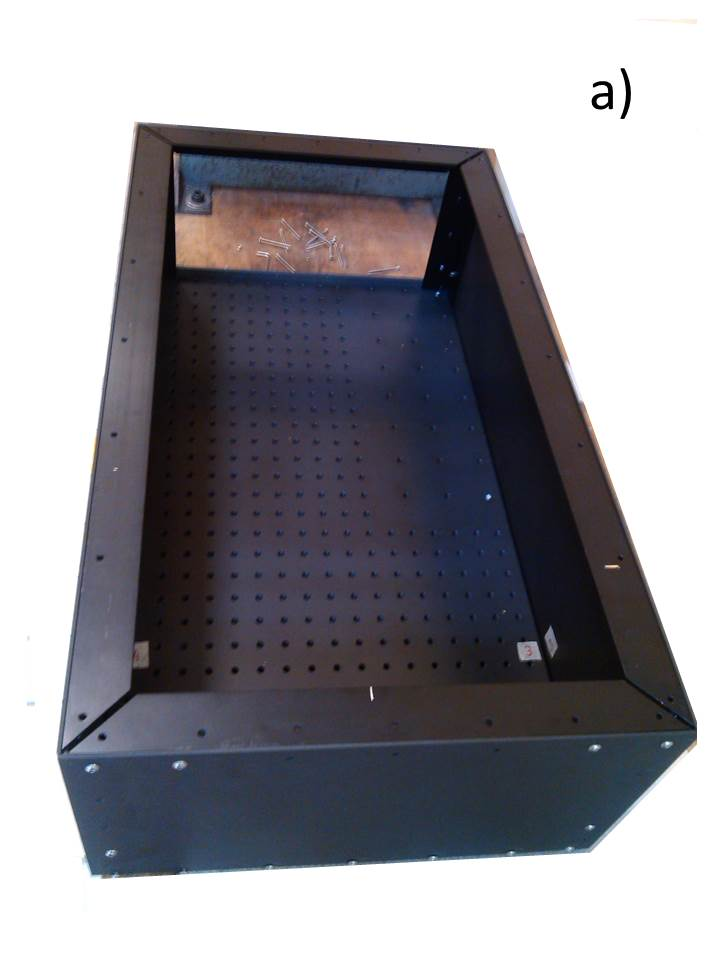
\includegraphics[width=5.8cm, height=9cm]{figures/Optics_box_1}
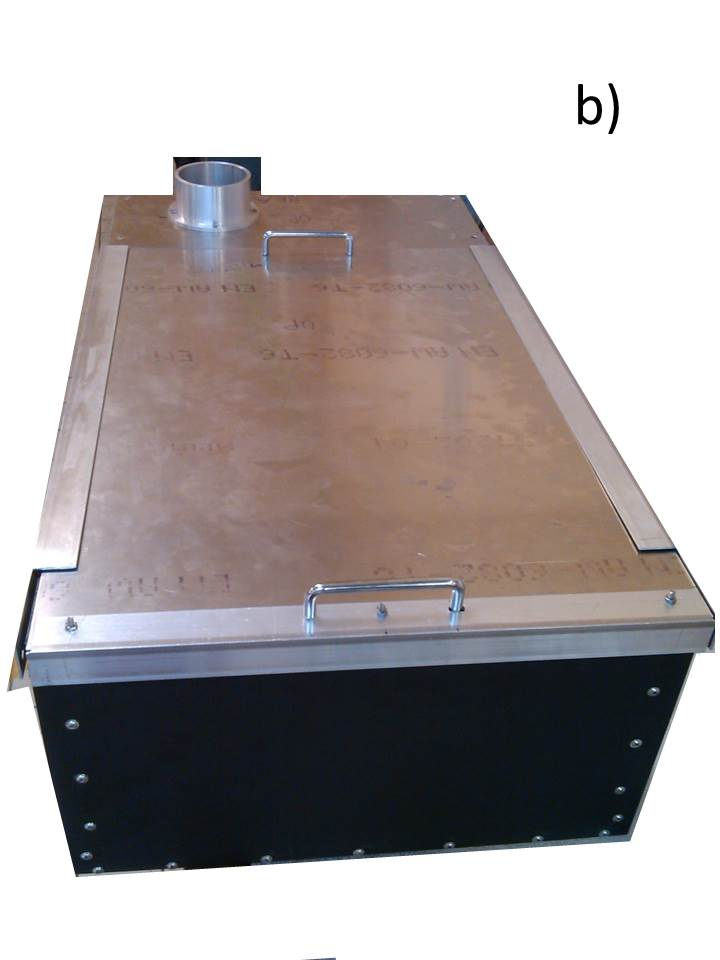
\includegraphics[width=5.8cm, height=9cm]{figures/Optics_box_2}
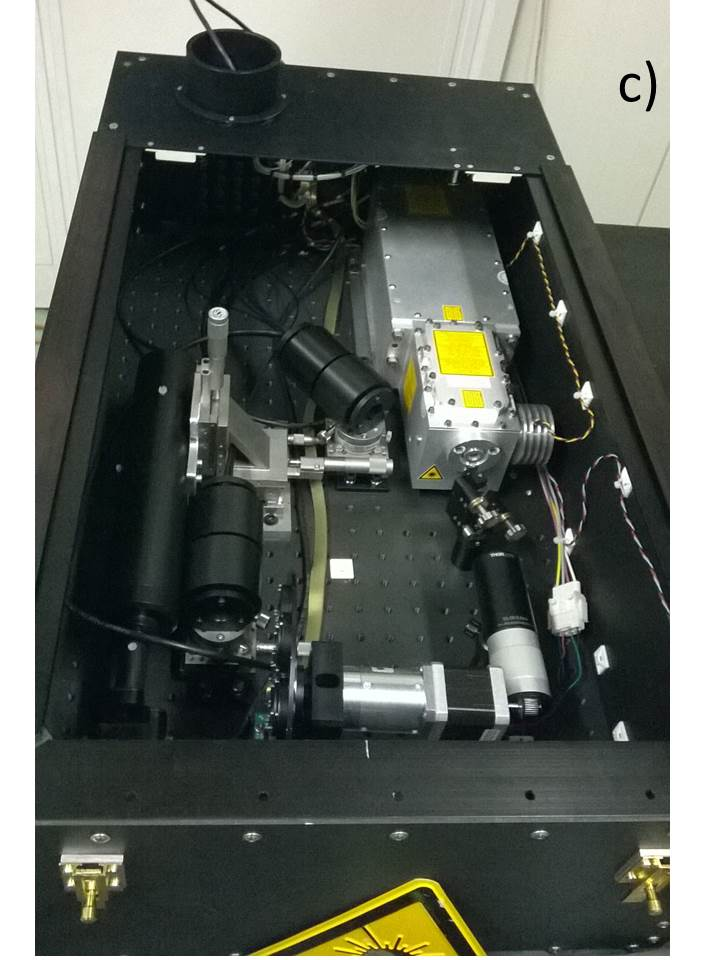
\includegraphics[width=5.8cm, height=9cm]{figures/Optics_box_3}
\caption{Pictures of the optics box: a) the thread hole grid of the box base; b) the
two section cover; c) the optical element arrangement before installation in the
ATLAS cavern.  
}\label{fig:x.0}
\end{center}
\end{figure}
%

A special black-anodized aluminum box contains the laser source and the main optical
elements to distribute light to the individual Tile modules, to filter the light
intesity and to monitor it. Various details are shown in figure \ref{fig:x.0} The
optics box has a 50 mm thick aluminum base plate with a 25 mm times 25 mm M6 hole
grid; this way, mechanical rigidity of the optical elements 
placed inside the box is insured with large flexibility for positioning the
individual pieces. The lateral walls of the box are made by thin (2 mm) aluminum
plates to
reduce the total weight of the box (about 20 Kg, when equipped with all the internal
elements). The rear panel has patch-panels with feed-throughs for electrical
connections or fiber connectors for the monitor signals. The top cover is divided
into two parts: a smaller section fixed to the walls with a 6 cm diameter hole to
allow the insertion of the 400 fiber bundle, and a sliding section to allow for
inspections.  An interlock system is used to break lasing in case of accidental
opening of the box. 

The optics box is inserted in a rack located in the underground ATLAS room called
USA-15 and mounted on an anti-vibration system. 
The same rack hosts the electronics 
to control the Laser\_II system and a patch panel containing about 400 fiber
couplers. The couplers receive in input the light from each fiber of the bundle
exiting the optics box; the fraction of light from each input fiber and transmitted
ahed is adjusted by acting on the coupler screws. The transmitted light is injected
into the individual 100 m long fibers feeding mixers inside each detector modules;
the mixers distribute the light to each PMT of module through short, variable lenght
clear fibers. . Pictures of the front and rear sides of the rack containing the
optics box, the electronics for the Laser\_II 
control and the fiber patch panel are shown in figure \ref{fig:x.1}.
% 
\begin{figure}[htb]
\begin{center} 
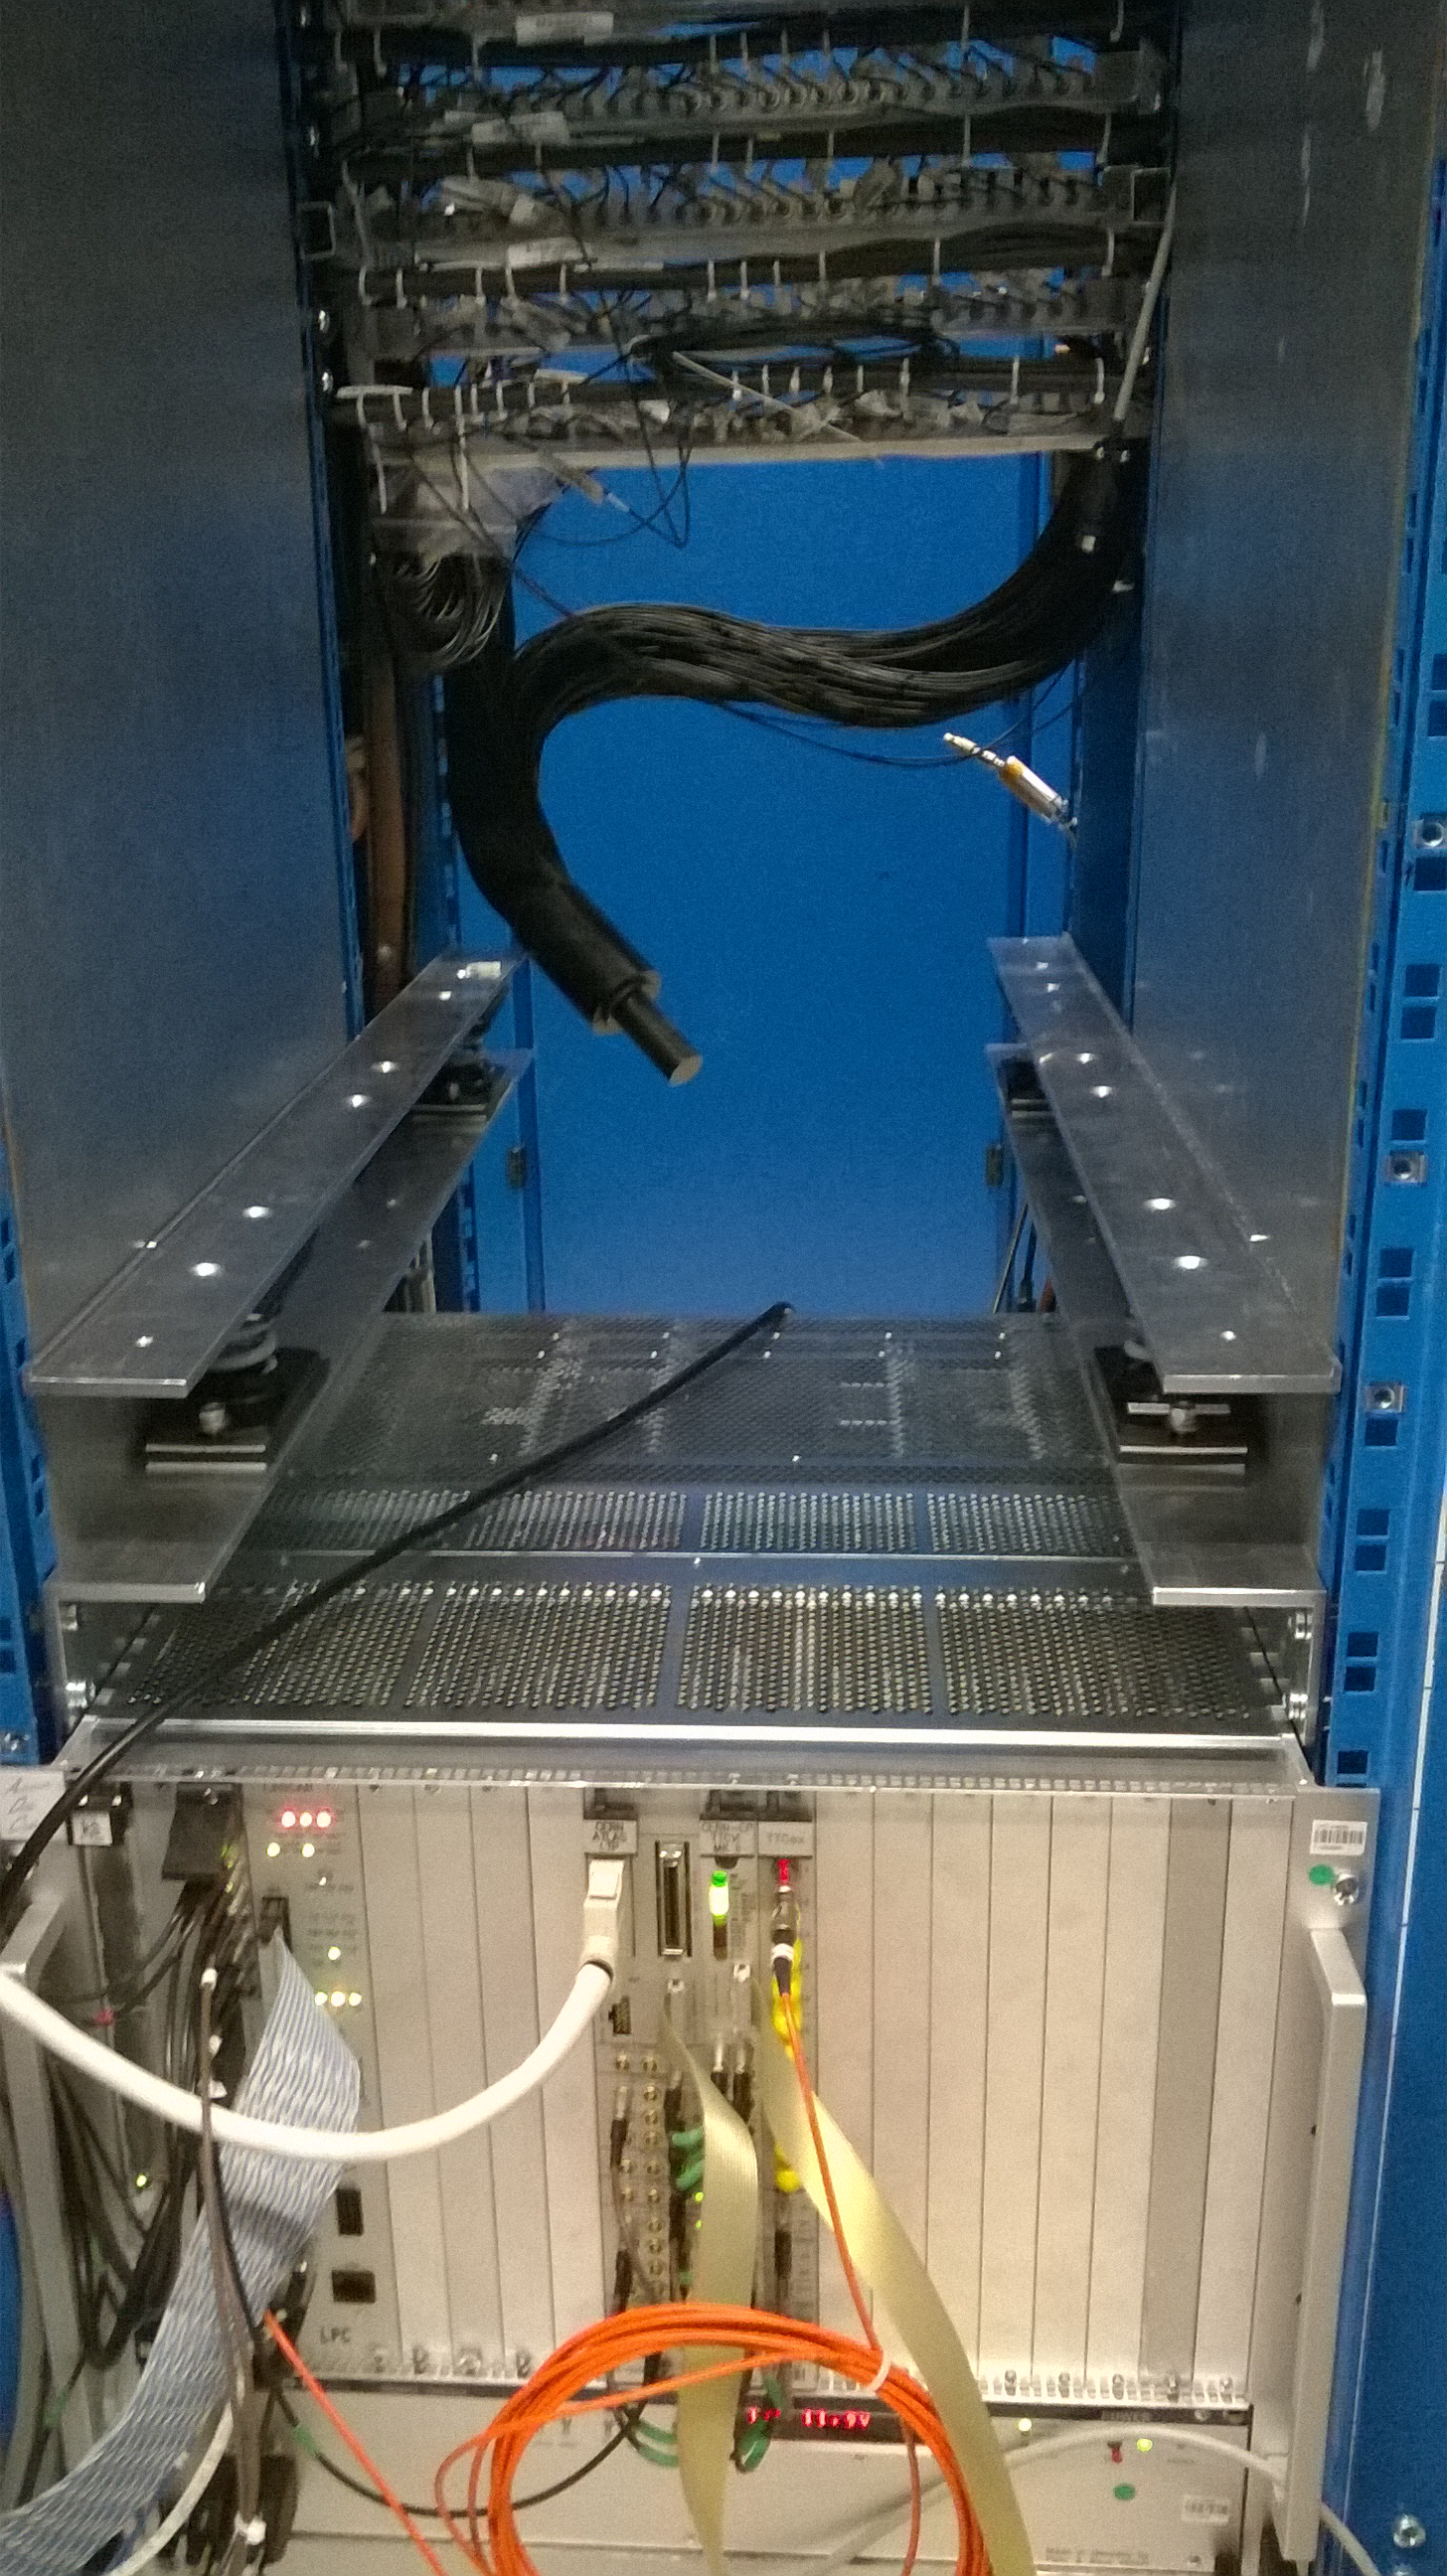
\includegraphics[width=5.8cm, height=9cm]{figures/WP_20141009_15_37_36_Pro}
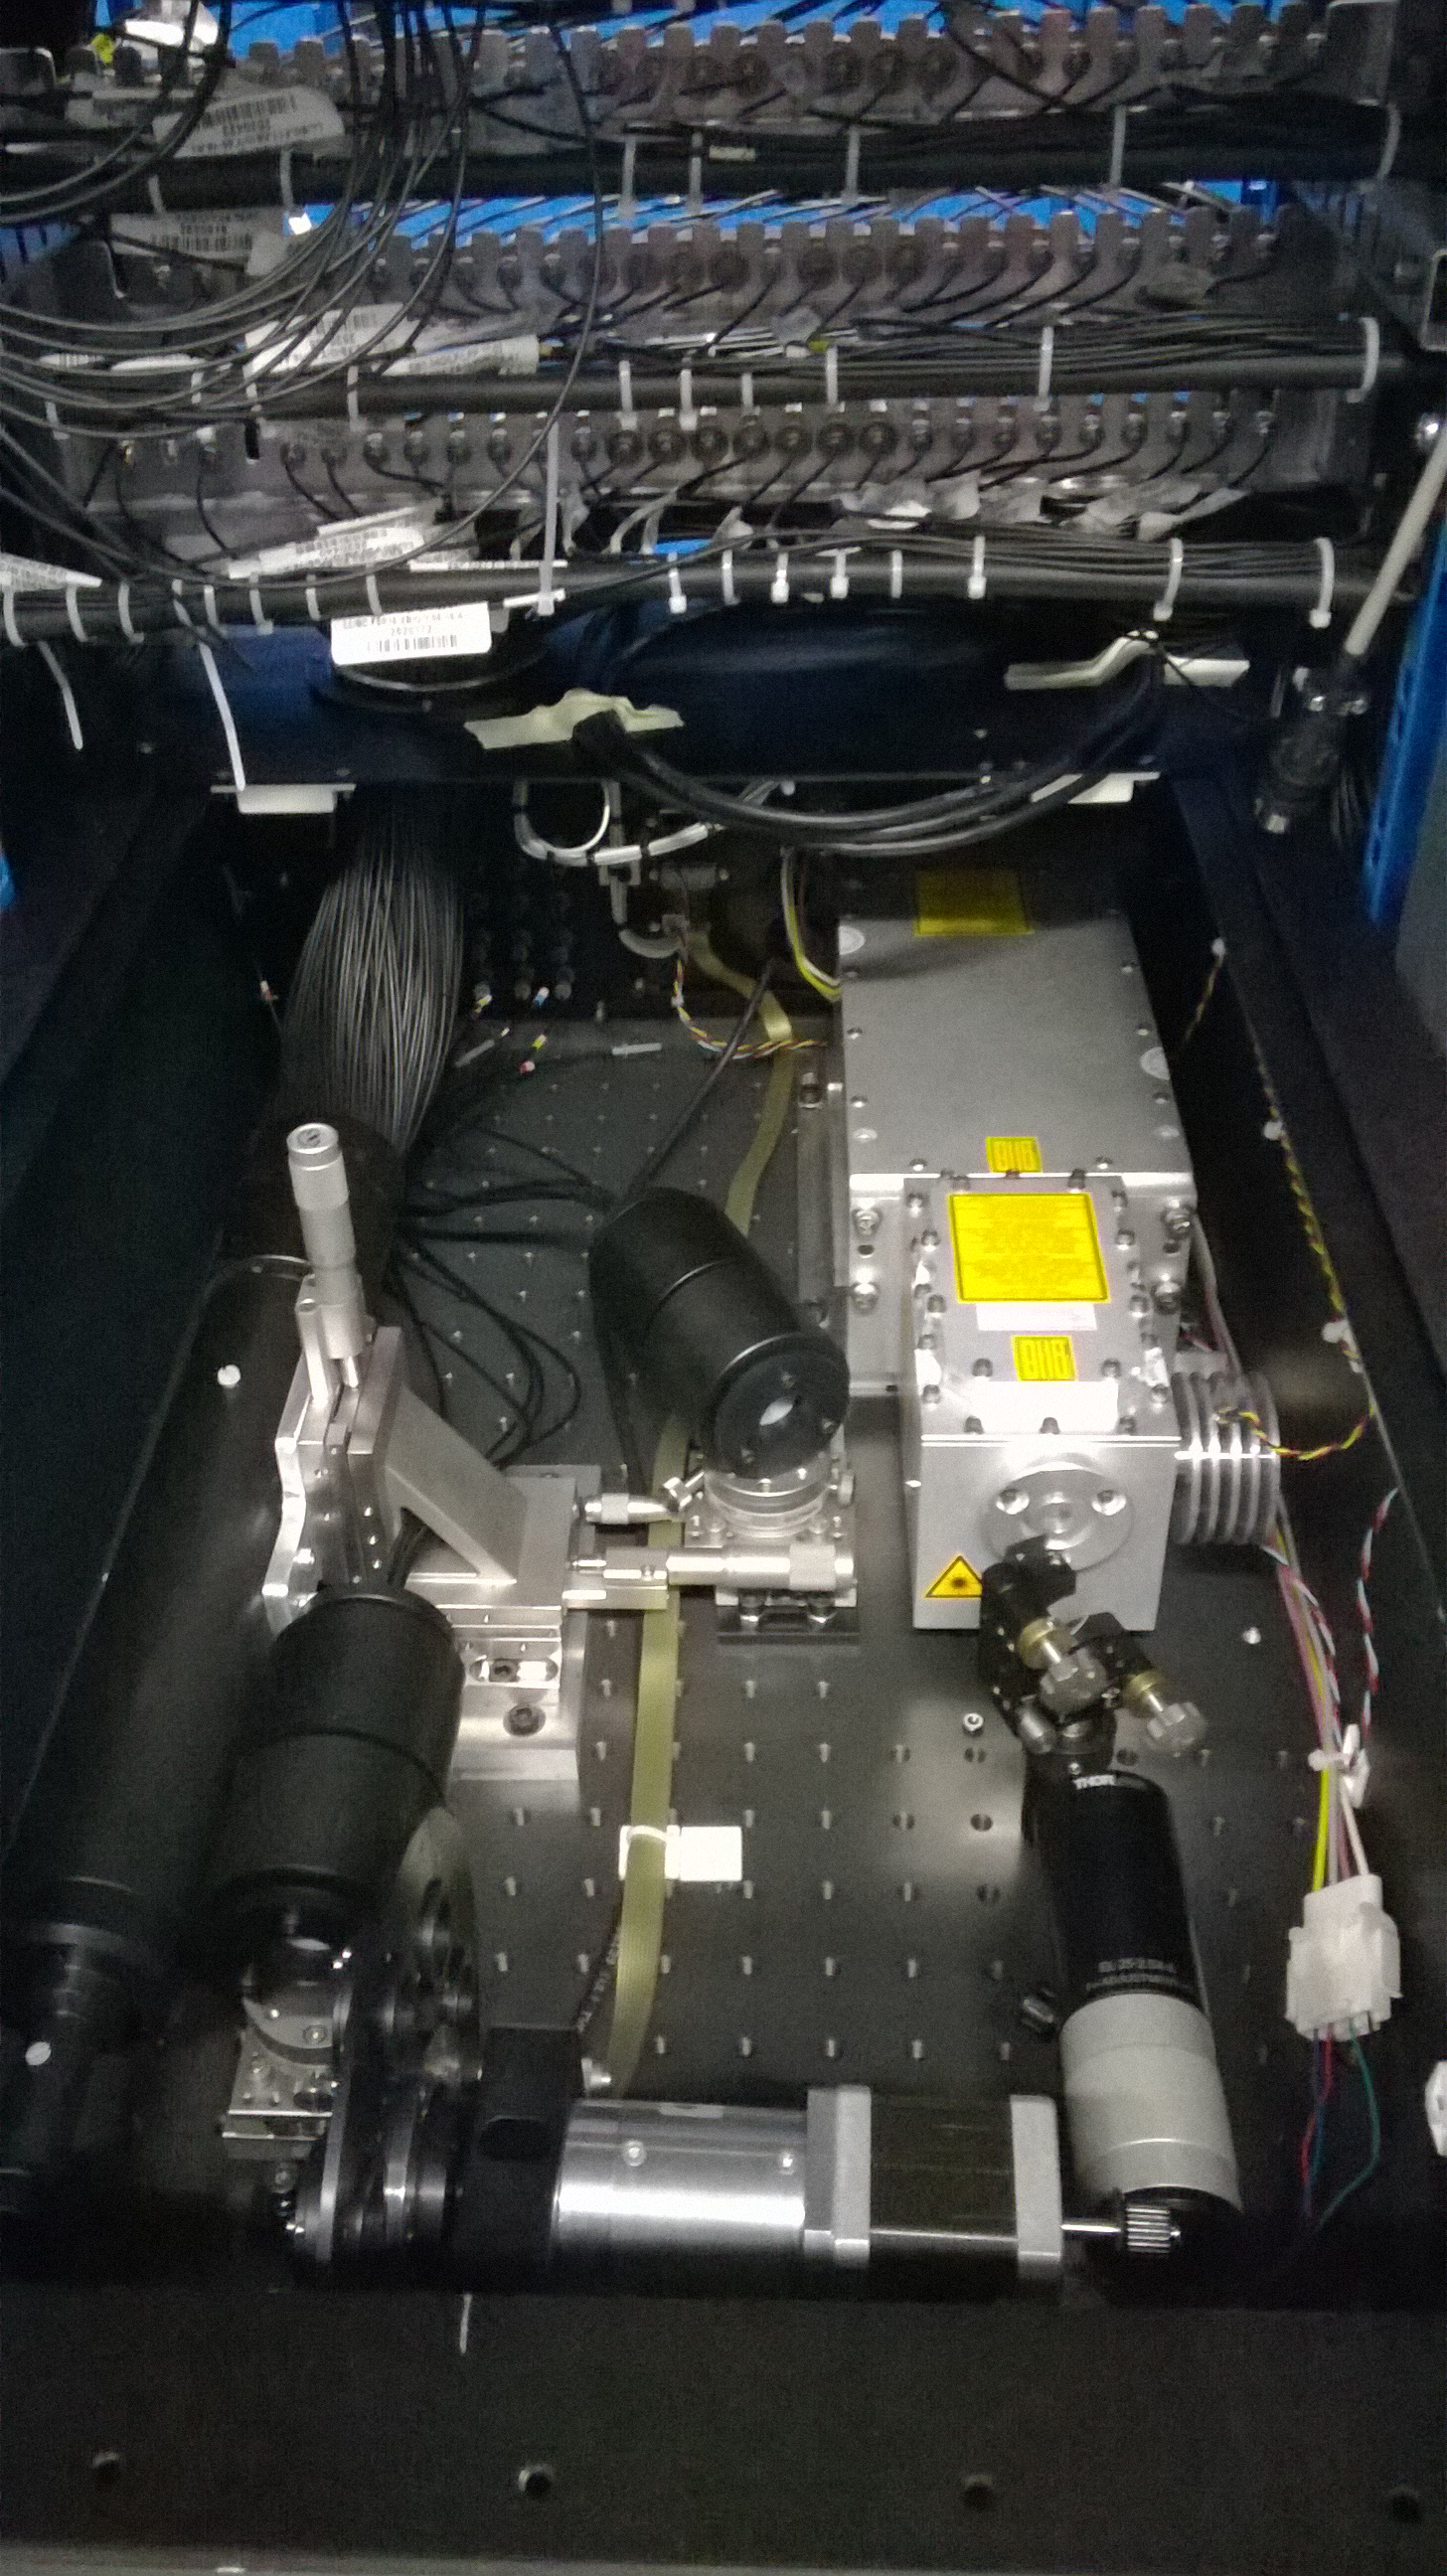
\includegraphics[width=5.8cm, height=9cm]{figures/WP_20141009_16_17_31_Pro}
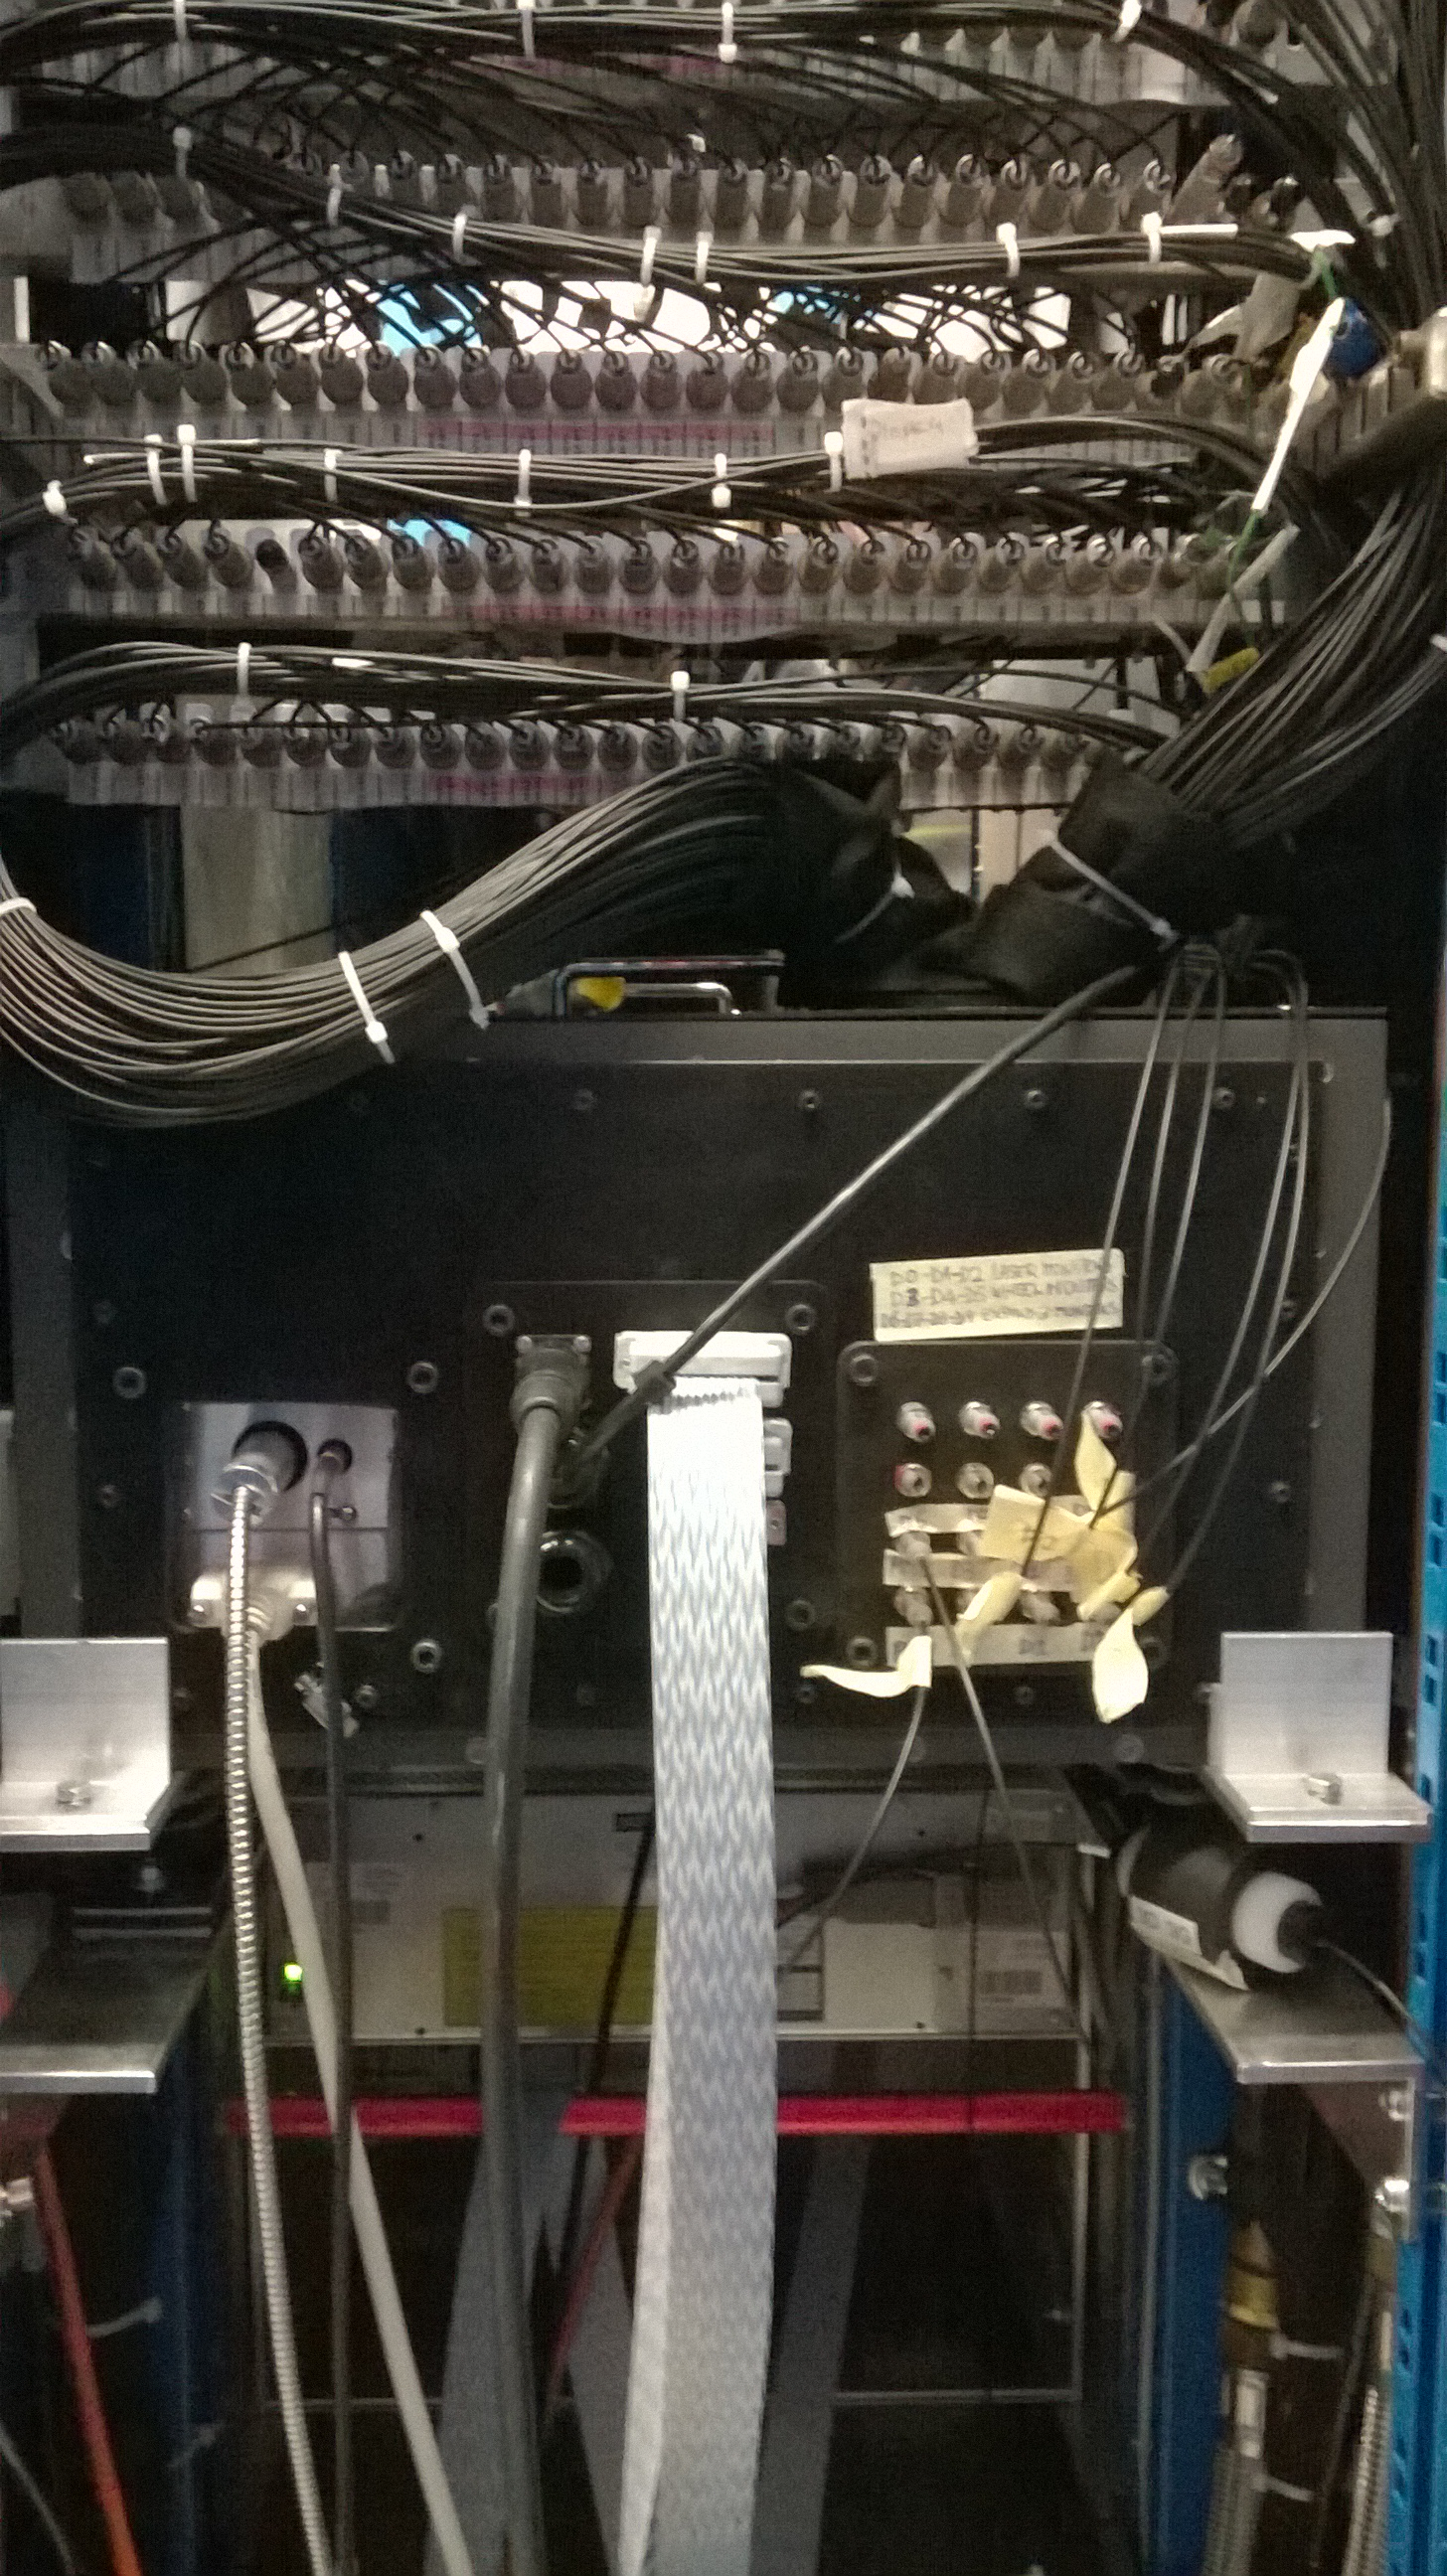
\includegraphics[width=5.8cm, height=9cm]{figures/WP_20141010_12_11_55_Pro}
\caption{Pictures of the installation of the optics box in the USA-15 room of the
ATLAS cavern; a) rails with anti-vibration springs to sustain the optics box; in the
rear the 400 fiber bundle pending from the connector patch-panel; b): the optics box
(cover removed) placed on the anti-vibration rails and coupled to the fiber bundle;
c) rear of the optics box; the fiber bundle exits from the top cover of the box;
feed-throughs are used in the box rear panel for passing laser control cables,
internal devices controls and fibers connected to the intensity monitors described
in the text.  
}\label{fig:x.1}
\end{center}
\end{figure}
%

The optical layout insidel to the optics box is shown in figure \ref{fig:x.2}. The
light source is a Q-switched, diode-pumped, solid state 
laser\footnote{Spectra Physics model Navigator $J40-BL6S-532Q$} with frequency
doubler ($\lambda = 532$ nm). The individual pulse energy 
and time width are about 50 $\mu$J and 10 ns, respectively. The maximum repetition
rate of the laser pulses is greater than 35 KHz, but in the operation modes 
used by the Laser\_II system, the repetition rate is set to 100 Hz for standard
laser calibration runs and at about 1 Hz for pulsing the laser 
in empty bunches during collisions in the LHC accelerator. 
% 
\begin{figure}[htb]
\begin{center} 
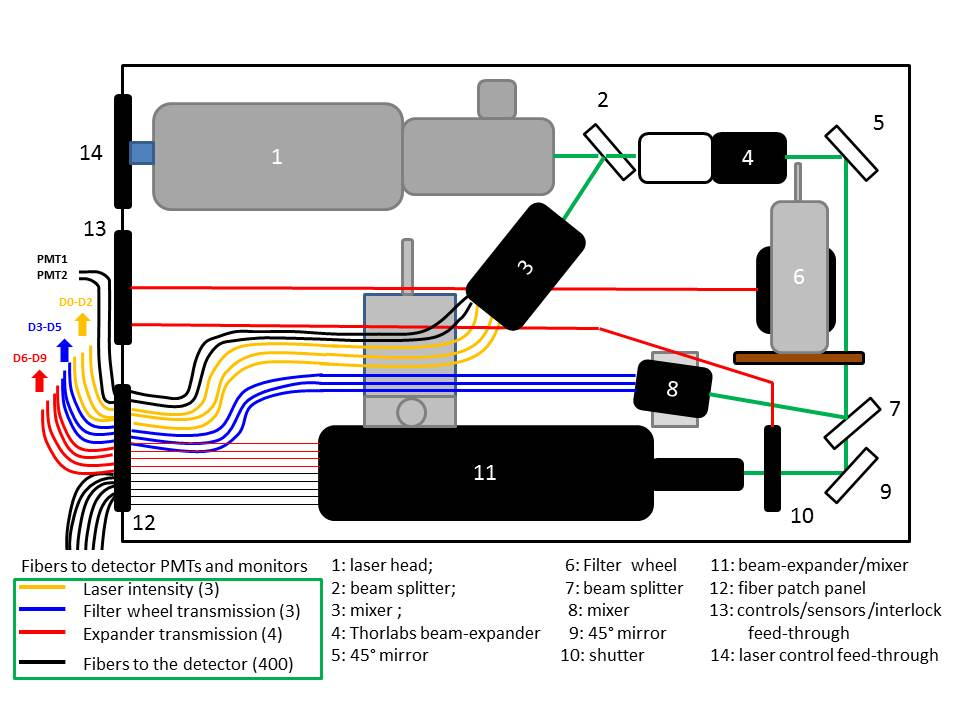
\includegraphics[width=16cm, height=11cm]{figures/Layout}
\caption{Optics box internal elements and optical paths; detailed description is
given in the text
}\label{fig:x.2}
\end{center}
\end{figure}
%

A small fraction (a few percent of the total intensity) of the beam exiting the
laser cavity is backwards fed onto a light mixer (position 3 in figure 
\ref{fig:x.2}) by a splitter placed on the optical path of the primary beam
(position 2 in figure \ref{fig:x.2}). Five clear fibers collect the light exiting
the mixer; two of these fibers are used to excite two PMTs contained in the $PMT
~box$ (section x.x), generating the trigger signal for the DAQ with proper delay
relative to the laser pulse. The other three fibers are routed to three monitor
diodes (D0-D2) located in the $Diode ~box$ (section x.x).  To avoid a too high laser
power density in the downstream optical elements, the beam spot is expanded from
about $700 ~\mu$m
(which is the dimension of the laser beam waist at the cavity exit) to about 2 mm by
a 2.5x beam-expander\footnote{Thorlabs model EL-25-2.5X-A} (position 4 in figure
\ref{fig:x.2}). A $45^{\circ}$ dielectric mirror (position 5) reflects the laser
beam towards the filter wheel (position 6) which hosts 8 neutral density filters
with different optical densities OD. The filter transmissions range between $100\%$
(no filter) to $0.3\%$ (OD=2.5). The transmission variation (a factor 300) times a
factor of about 6 for the range of intensities where the laser operation is stable,
provides a global factor of about 2,000 for the span of the pulse energy reaching
the individual detector PMTs, i.e. detector PMT responses can be calibrated in the
equivalent energy range [500 MeV, 1 TeV].

A picture of the filter wheel is shown in figure \ref{fig:x.3}a) and the filter
positions on the wheel are shown in figure \ref{fig:x.3}b). The filter wheel is
moved by a stepping motor with remote numeric control and the filter position is
controlled by a combined opto-mechanical system which allows for 
position accuracy of about  $xxx ~\mu$m. The driver of the filter wheel is located
in the PMT box.
% 
\begin{figure}[htb]
\begin{center} 
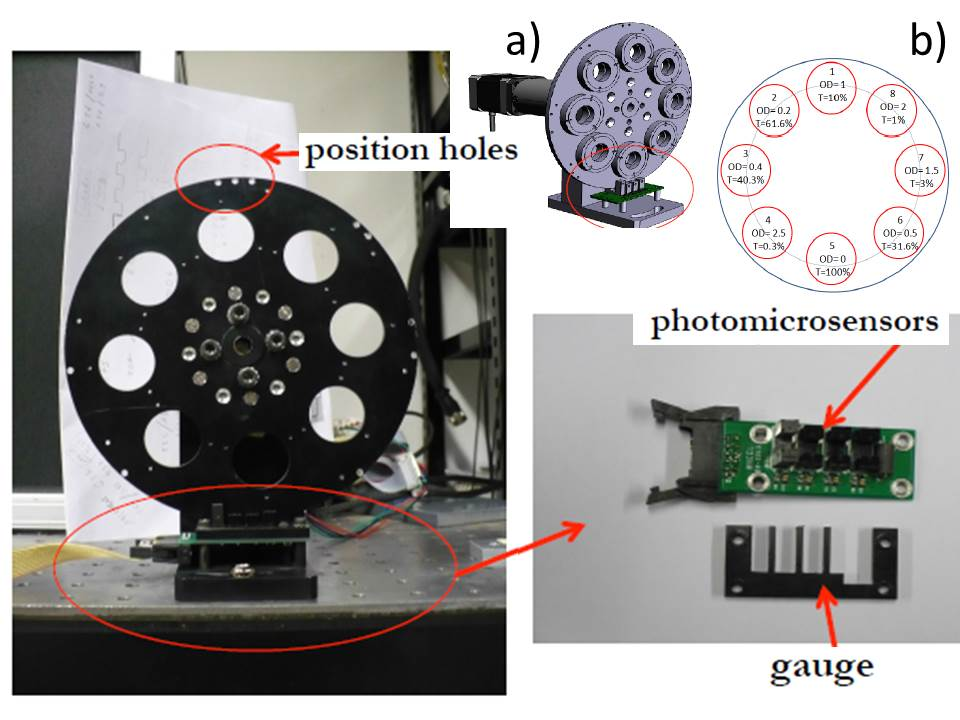
\includegraphics[width=16cm, height=11cm]{figures/Filter_wheel}
\caption{Filter wheel geometry
}\label{fig:x.3}
\end{center}
\end{figure}
%

 A small fraction (a few percent of the total intensity) of the light transmitted by
the selected filter on the wheel is fed onto a light mixer (position 8) by a
splitter placed downstream the wheel (position 7). Both mixers in positions 3 and 8
are assembled as a wafer of a PMMA optical guide between silica diffusers.
Three clear fibers collect the light exiting the mixer and they are routed onto
three monitor diodes (D3-D5) located in the $Diode ~box$. As in the case of the
first mixer (position 3), the redundant information from photodiodes monitoring the
light intensity at the same point in the optical line allows to control the relative
stability of their response. 

A second $45^{\circ}$ dielectric mirror (position 9) reflects the laser beam towards
the final beam-expander (position11). A remotely controlled shutter (position 10) is
placed in between the mirror and the final beam-expander. The shutter is normally
kept closed during beam collisions to protect the detector PMTs against accidental
lasing which could occur in case of failure in the laser control system. When the
shutter is closed, filter transmission tests and monitor response checks of diodes
D0 to D5 can be performed even during normal data taking. The shutter is open only
when the standard laser calibration runs are performed, tipically every two-three
days during short collision stops. The full calibration procedure, i.e. the sequence
of calibrations internal to the laser system and described in section x.x and the
laser calibration of the detetcor PMTs, takes about one hour. The shutter is also
open during stable collision periods, whenever a control of the timing for the
detector PMT responses is required; in this case, laser pulses are sent at very low
frequency (1 Hz) in the time window corresponding to
beam empty bunches. 

The main element of the optical line is the final beam-expander (position 11). The
task of this element is to uniformely distribute the incoming light, which has a
beam waist of about 2 mm on the surface of the collar of the 400 fiber bundle which
is coupled to the exit of this element. The 400 fiber heads are packed inside a
plastic collar, after removal of the fiber external protection, in a circular bundle
30 mm in diameter.  In order to minimize any fiber-to-fiber relative change in the
amount of collected light in case of pointing variation of the laser beam, a quite
complex optical system was designed and its constructive parameters were tuned
during a long commissioning period.  The detailed scheme of this element is shown in
figure \ref{fig:x.4}.
% 
\begin{figure}[htb]
\begin{center} 
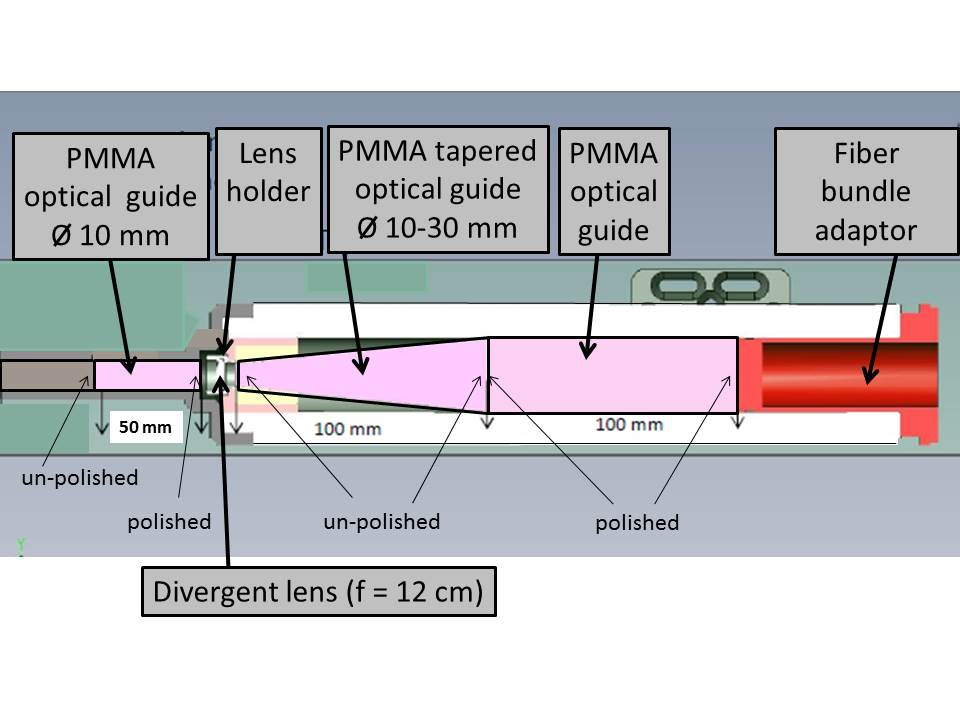
\includegraphics[width=13cm, height=9cm]{figures/Beam_expander}
\caption{Beam-expander geometry
}\label{fig:x.4}
\end{center}
\end{figure}
%

The light entering the beam-expander is first diffused by the un-polished face of a
PMMA cylinder, 10 mm in diameter and 50 mm long. The beam divergence is further
increased by a divergent lens (f=12 cm) and the optical paths are mixed by the
additional diffusion introduced by the two un-polished faces of a tapered PMMA
optical guide. The wider face diameter of this guide is 30 mm as that of the last
PMMA cylinder which is used to improve the light mixing at
the entrance of the 400 fiber bundle collar. The geometry of the beam-expander was
tuned to get an acceptable compromise between the minimization
of the light loss (30$\%$ at each un-polished surface on average) and the
minimization of the fluctuations of the fiber-to-fiber light collection at the
expander exit, induced by pointing effects of the laser beam. The non-uniformity of
the light collected at the expander exit was measured to be below 1$\%$ for
displacements of the laser beam entry point on the expander up to 1 mm with respect
to the axis of the optical guides and lens. The beam-expander is fixed to the optics
box base with a X-Z mount system which allows for accurate positioning through
micrometric actuators.

Four fibers, randomly picked-up among the 400 of the big bundle faced to the
expander exit, are coupled to four monitor diodes (D6-D9). The information from
these monitors is used to control the stability of the total amount of light
transmitted by the full optical system and the stability of the relative fraction of
light collected by each individual fiber in the bundle.

The performances of the optical system described in this section were studied during
a long design and test period in a dedicated ATLAS Tile laboratory on the surface in
the CERN site during year 2014. The system was installed in the service room in the
ATLAS cavern and coupled to the existing 400 fiber bundle and to the other pieces of
the whole new Laser$\_$II system in Autumn 2014. The performances of the optical
part of the system were measured again during the full system commissioning period
in the first half of 2015 until the first run II collisions of the LHC. A summary of
the typical performances of the optical system obtained in the commissioning period
and in the first weeks of regular data taking during collisions is given in section
x.x.  

